\documentclass[11pt,a4paper]{scrartcl}
\typearea{12}
\usepackage{graphicx}
\usepackage{pstricks}
\usepackage{listings}

\usepackage{tikz}
\usepackage{tikzscale}
\usepackage{pgfplots}

\usepackage{pgf}
\usepackage[utf8]{inputenc}
\usetikzlibrary{arrows,automata}
\usetikzlibrary{positioning}


\tikzset{
    neuron/.style={
           rectangle,
           rounded corners,
           draw=black, very thick,
           inner sep=2pt,
           text centered,
           },
}


\tikzset{
    gc/.style={
           rectangle,
           rounded corners,
           draw=red, very thick,
           inner sep=2pt,
           text centered,
           },
}


\tikzset{
    io/.style={
           rectangle,
           rounded corners,
           draw=green, very thick,
           inner sep=2pt,
           text centered,
           },
}


\tikzset{
    on/.style={
           circle,
           draw=red, very thick,
           inner sep=4pt,
           fill=red!45,
           },
}


\tikzset{
    off/.style={
           circle,
           draw=blue, very thick,
           inner sep=4pt,
           text centered,
           },
}



\pgfplotsset{compat=1.8}


\lstset{language=python}
\pagestyle{headings}
\markright{Computational Neuroscience - 13 reinforcement}
\begin{document}

\subsection*{Introduction}
These notes are about reinforcement learning.
\subsection*{Action selection}

Classical conditioning tests responses using an experimental paradigm
which in its reliability differs from the real world. The bell rings
and the dog gets fed, little in our lives offers this sort of
reliability, we hear a bell and we know we need to leave the building
and can guess the probability that there is a fire or that we'll get
into trouble for not taking part in a drill; we evaluate based on
probabilities and on estimated likelihoods of various future harms and
rewards. Action selection relates to the problem of choosing actions
in this uncertain and probabilistic world. The basal ganglia is
considered the seat of action selection.

The classic experiment in action selection is described in
\cite{DawEtAl2006a}; it involves one-arm-bandits, modelled on the
gambling machines you find in amusement arcades and casinos. The
player is presented with a choice of four one-arm-bandits and chooses
one, they play and receive a reward; they then choose again. The mean
rewards are adjusted over time. The question is, how does the player
choose which bandit to play and how to the make sure to continue
exploring the other bandits in case they become better as the means
are changed.

One strategy is to estimate rewards and match choice probability to
these estimates. Hence, say $m_i$ is the estimated reward for action
$i$; then the probability of choosing $i$ is
\begin{equation}
p_i=\frac{\exp{\beta m_i}}{\sum_j\exp{\beta m_j}}
\end{equation}
where $\beta$ is a \lq{}choosiness\rq{} or exploration parameter. If
$\beta=0$ then all actions are chosen with equal probability and there
is little discrimination; if $\beta$ is very large, the action with
the highest estimated reward is chosen with probability near one, and
there is little exploration. Of course $m_i$ is updated based on
outcome, 
\begin{equation}
m_i\rightarrow m_i+\eta \delta
\end{equation}
where $\eta$ is a learning rate and 
\begin{equation}
\delta = r-m_i 
\end{equation}
is the error in the expected reward.


\begin{figure}
\begin{center}
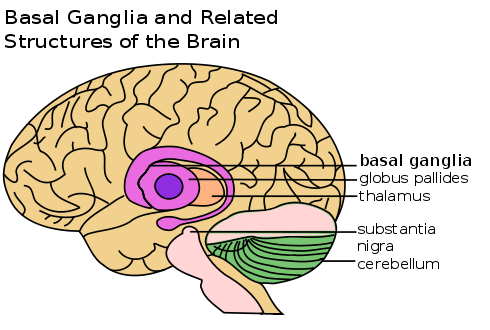
\includegraphics[width=10cm]{basal_ganglia_wikipedia.png}%
\end{center}
\caption{The basal ganglia. This picture is slightly misleading since
  it looks like the basal ganglia is on the surface of the brain when
  it is on the inside, it is as if the beige parts of the picture,
  showing the cortex, are transparent. It also labels the globus
  pallides and substantia nigra separately as if they were distinct
  from the basal ganglia, when they are part of it. [Picture from
    wikipedia]\label{fig:basal_ganglia}}
\end{figure}

\subsection*{Basal ganglia}

The basal ganglia, Fig.~\ref{fig:basal_ganglia}, is a collection of
sub-cortical brain areas, or nuclei, found near the center of the
brain and connected to the cortex, thalamus and brain stem. It is
thought to be important in decision making, action selection and in
the regulation of some routine behaviors, like eye movements. Its
constituent nuclei include the striatum, the globus pallidus, the
substantia nigra, the nucleus accumbens, and the subthalamic
nucleus. These are all quiet complex with different, sometimes very
distinctive, neurons; they are frequently divided still further, so,
for example, in models of basal ganglia the globus pallidus is divided
to the excitatory part of globus pallidus and the inhibitory. There
are also channels in the basal ganglia, there are parts of each
nucleus that correspond to different muscles and different parts of
the body.

The basal ganglia has lots of inhibitory projections, so it is thought
it acts mostly switching off inhibition. In other words, there are
cells which inhibit muscles and the basal ganglia is thought to work
by, in turn, inhibiting those cells, see Fig.~\ref{fig:inhib} for a
sketch of this mechanism.

\begin{figure}
\begin{center}
\begin{tabular}{lp{1cm}l}
\textbf{A}&&\textbf{B}\\
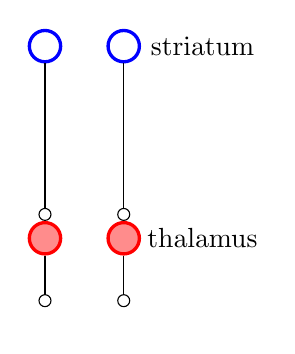
\begin{tikzpicture}
\node[off](s1){};
\node[off,right of =s1](s2){};
\node[right of = s2,align = left](s){striatum};
\node[on,below = 2cm of s1](t1){};
\node[on,below = 2cm of s2](t2){};
\node[right of = t2,align=left](t){thalamus};
\node[below of =t1](bt1){};
\node[below of =t2](bt2){};
\path (s1)edge[-o](t1);
\path (s2)edge[-o](t2);
\path (t1)edge[-o](bt1);
\path (t2)edge[-o](bt2);
\end{tikzpicture}
&&
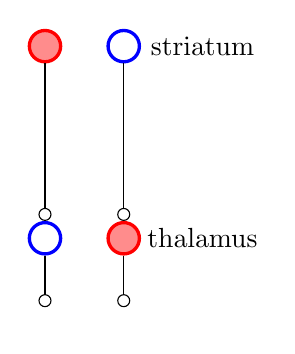
\begin{tikzpicture}
\node[on](s1){};
\node[off,right of =s1](s2){};
\node[right of = s2,align = left](s){striatum};
\node[off,below = 2cm of s1](t1){};
\node[on,below = 2cm of s2](t2){};
\node[right of = t2,align=left](t){thalamus};
\node[below of =t1](bt1){};
\node[below of =t2](bt2){};
\path (s1)edge[-o](t1);
\path (s2)edge[-o](t2);
\path (t1)edge[-o](bt1);
\path (t2)edge[-o](bt2);
\end{tikzpicture}
\end{tabular}
\end{center}
\caption{The basal ganglia controls by disinhibition. In \textbf{A} the thalamic neurons inhibit the muscles; however in \textbf{B} one of the basal ganglia neurons has become active, it inhibits a thalamic neuron, disinhibiting the left muscles. \label{fig:inhib}}
\end{figure}

\subsection*{Model of action selection in the basal ganglia}

This circuit is very similar to the one introduced in classical
conditioning, however, although dopamine plays a similar role,
describing the error, a different set of dopaminergic neurons may be
involved, the dopaminergic neurons of the substantia nigra (SN). The model
is represented in Fig.~\ref{fig:full_circuit}.

\begin{figure}
\begin{center}
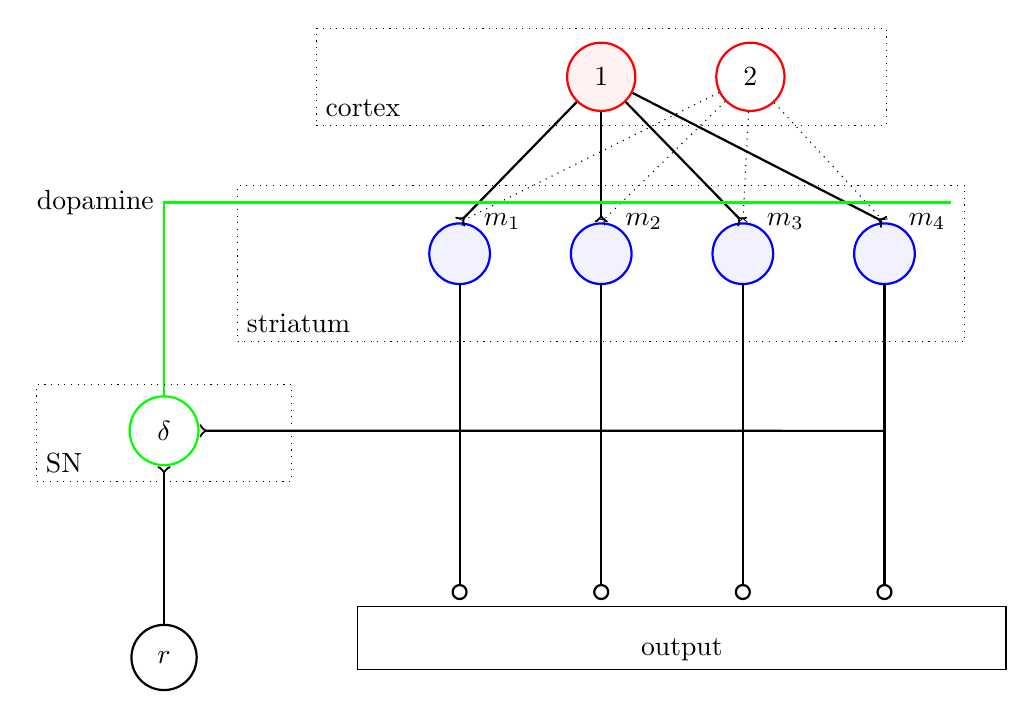
\begin{tikzpicture}
\node[text width=7cm, text height=1cm, draw=black, dotted](SC){cortex};
\node[align=center,text width=0.5cm,circle,draw=red, thick, fill=red!5](x1){$1$}; 
\node[align=center,text width=0.5cm,circle,draw=red, thick, fill=red!0, right = 1cm of x1](x2){$2$};
\node[text width=9cm, text height=1.75cm, draw=black, dotted,below =0.75cm of SC](St){striatum}; 
\node[text width=0.5cm,circle,draw=blue, thick, fill=blue!5,below = 1.4cm of x1](w2){};
\node[above right = -0.1cm and -0.1cm of w2]{$m_2$};
\node[align=center,text width=0.5cm,circle,draw=blue, thick, fill=blue!5, left = 1cm of w2](w1){};
\node[above right = -0.1cm and -0.1cm of w1]{$m_1$};
\node[right=0.5cm of w2](v){};
\node[text height=0.5cm,text width=8cm, draw=black,below=4.35cm of v,align=center]{output};
\node[align=center,text width=0.5cm,circle,draw=blue, thick, fill=blue!5, right = 1cm of w2](w3){};
\node[align=center,text width=0.5cm,circle,draw=blue, thick, fill=blue!5, right = 1cm of w3](w4){};
\node[above right = -0.1cm and -0.1cm of w3]{$m_3$};
\node[above right = -0.1cm and -0.1cm of w4]{$m_4$};
\path (x1) edge[thick,-<] (w1.north);
\path (x1) edge[thick,-<] (w2.north);
\path (x1) edge[thick,-<] (w3.north);
\path (x1) edge[thick,-<] (w4.north);
\path (x2) edge[dotted,-<] (w1.north);
\path (x2) edge[dotted,-<] (w2.north);
\path (x2) edge[dotted,-<] (w3.north);
\path (x2) edge[dotted,-<] (w4.north);


\node[below= 2cm of v](belowv){};
\node[align=center,text width=0.5cm,circle,draw=green, thick, left = 6cm of belowv](delta){$\delta$};

\node[below = 4cm of w1](bw1){};
\node[below = 4cm of w2](bw2){};
\node[below = 4cm of w3](bw3){};
\node[below = 4cm of w4](bw4){};

\draw[thick,-<] (w4) -- ++(0,-2.25)--(delta);

\path (w1) edge[thick,-o] (bw1);
\path (w2) edge[thick,-o] (bw2);
\path (w3) edge[thick,-o] (bw3);
\path (w4) edge[thick,-o] (bw4);


\node[align=center,text width=0.5cm,circle,draw=black, thick, below= 2cm of delta](r){$r$};
\path (r) edge[thick,-<] (delta);
\draw[thick,green] (delta) --++ (0,2.9)node[left,black]{dopamine} --++ (10,0); 
\node[text width=3cm, text height=1cm, draw=black, dotted,above =1.8cm of r](SN){SN}; 

\end{tikzpicture}
\end{center}
\caption{A diagram of the action selection circuit. The cortical input, labeled \lq{}1\rq{} excites some neurons in the striatum; the synapses have strengths corresponding to the estimated rewards and, in this simple model, this determines the amount of activity in the post-synaptic neuron, these neurons in turn disinhibit neurons in the output, allowing the corresponding muscles to move, the difference between this activity and the reward is represented by dopamine and causes synaptic changes at the cortico-striatal synapses.\label{fig:full_circuit}}
\end{figure}


Evidence for this model is provided by recordings from human patients
in \cite{ZaghloulEtAl2009a}; recordings where taken from Parkinson's
patients during surgery for deep brain stimulation. The subjects
played a one-armed-bandit type game, this version involved drawing
cards from two decks, one had a 0.35 chance of reward, the other
0.65. As shown in Fig.~\ref{fig:human} there is increased activity in
SN when there is a reward from the 0.35 card and a decrease in
activity when there is no reward from the 0.65 card.


\begin{figure}
\begin{center}
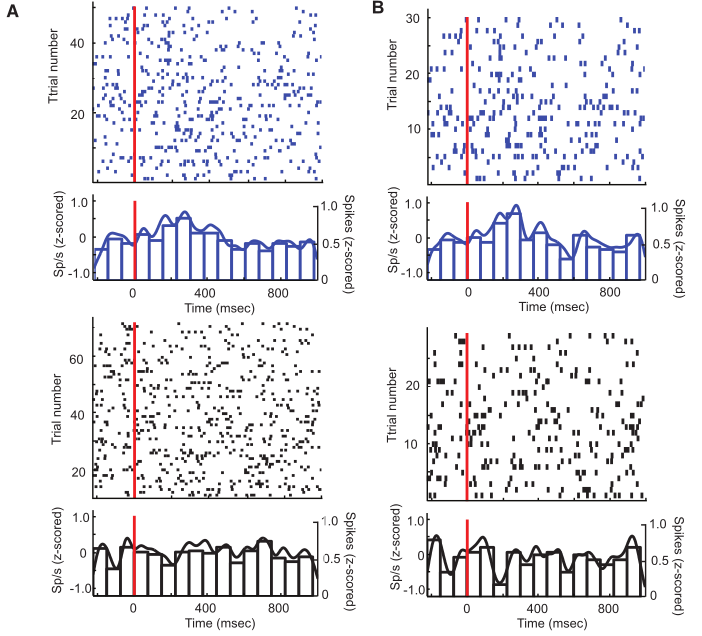
\includegraphics[width=10cm]{human.png}%
\end{center}
\caption{Response from SN in one patient during a game of chance from \cite{ZaghloulEtAl2009a}, The top, blue, graphs shows increased activity during an expected reward, the bottom, black, shows decreased when a reward is expected, but doesn't appear. \label{fig:human}}
\end{figure}

Very direct evidence is provided in
\cite{ReynoldsHylandWickens2001a}. A clever two phase experiment is
used to measure changes in synaptic weight directly. In the first
phase SN neurons are stimulated electrically in rat during a lever
press task; the optimal stimulation for learning is found; during the
second phase the rat is anaesthetised and the cortex, striatum and SN
are stimulated directly and the synaptic weights are measured. It is
found that the cortico-striatal weights increase during simulated
learning.

\subsection*{Actor-critic model}

The is plenty of evidence for a SN dopaminergic error signal. However,
the connectivity the model involves is not consistent with the
connectivity actually observed. The actor-critic fixes this; it
divides the striatum into two parts, the large \lq{}actor\rq{} part
that guides action and is associated with the dorsal, that is front,
part of the striatum and a smaller \lq{}critic\rq{} part used to
calculate reward; this is associated with the ventral, that is lower,
part. This circuit is sketched in Fig.~\ref{fig:actor_critic}. In the
model actions are selected according to the expected reward $m_i$, an
error is calculated using $\delta=r-w$ and both $w$ and $m_i$ are
updated
\begin{equation}
m_i\rightarrow m_i +\eta \delta
\end{equation}
and 
\begin{equation}
w\rightarrow w +\eta \delta.
\end{equation}
There is some proof for this model provided in
\cite{ODohertyEtAl2004a}. In this paper subjects play a
one-armed-bandit-style game under two conditions, one where the
computer chooses, one where the subject chooses. In both the ventral
striatum is engaged, but the dorsal striatum is only engaged when the
subject chooses.

\begin{figure}
\begin{center}
\begin{tikzpicture}
\node[text width=7cm, text height=1cm, draw=black, dotted](SC){cortex};
\node[align=center,text width=0.5cm,circle,draw=red, thick, fill=red!5](x1){1}; 
\node[align=center,text width=0.5cm,circle,draw=red, thick, fill=red!0, right = 1cm of x1](x2){2};
\node[text width=11.5cm, text height=2.5cm, draw=black, dotted, below = 0.5cm of SC,align=right](St){striatum}; 
\node[text width=2.4cm, text height=1.75cm, draw=black, dotted,left =0.35cm of w2](StC){critic}; 
\node[text width=6cm, text height=1.75cm, draw=black, dotted,right =0.15cm of StC,align=right](StA){actor}; 
\node[align=center,text width=0.5cm,circle,draw=blue, thick, fill=blue!5,below = 1.4cm of x1](w2){}; 
\node[align=center,text width=0.5cm,circle,draw=blue, thick, fill=blue!5, left = 1.4cm of w2](w1){};
\node[right=0.5cm of w2](v){};
\node[text height=0.5cm,text width=5cm, draw=black,below=4.1cm of w3,align=center]{output};
\node[align=center,text width=0.5cm,circle,draw=blue, thick, fill=blue!5, right = 1cm of w2](w3){};
\node[align=center,text width=0.5cm,circle,draw=blue, thick, fill=blue!5, right = 1cm of w3](w4){};
\path (x1) edge[thick,-<] (w1.north);
\path (x1) edge[thick,-<] (w2.north);
\path (x1) edge[thick,-<] (w3.north);
\path (x1) edge[thick,-<] (w4.north);
\path (x2) edge[dotted,-<] (w1.north);
\path (x2) edge[dotted,-<] (w2.north);
\path (x2) edge[dotted,-<] (w3.north);
\path (x2) edge[dotted,-<] (w4.north);


\node[below= 2cm of v](belowv){};
\node[align=center,text width=0.5cm,circle,draw=green, thick, left = 6cm of belowv](delta){$\delta$};

\node[below = 4cm of w2](bw2){};
\node[below = 4cm of w3](bw3){};
\node[below = 4cm of w4](bw4){};

\draw[thick,-<] (w1) -- ++(0,-2.25)--(delta);


\path (w2) edge[thick,-o] (bw2);
\path (w3) edge[thick,-o] (bw3);
\path (w4) edge[thick,-o] (bw4);


\node[align=center,text width=0.5cm,circle,draw=black, thick, below= 2cm of delta](r){$r$};
\path (r) edge[thick,-o] (delta);
\draw[thick,green] (delta) --++ (0,2.9) --++ (10,0); 
\node[text width=3cm, text height=1cm, draw=black, dotted,above =1.8cm of r](SN){SN}; 

\node[above right = -0.1cm and -0.1cm of w1]{$m_1$};
\node[above right = -0.1cm and -0.1cm of w2]{$m_2$};
\node[above right = -0.1cm and -0.1cm of w3]{$m_3$};
\node[above right = -0.1cm and -0.1cm of w4]{$m_4$};

\end{tikzpicture}
\end{center}
\caption{A diagram of the actor-critic circuit: there is a separate pathway for directing, that is disinhibiting, action and for calculating error.\label{fig:actor_critic}}
\end{figure}

\subsection*{Rewards and harms}
One problem with these models is that all the projections from the
cortex to the striatum are excitatory, so all the $m_i$ must be
positive; this doesn't reflect the state of the world, there are
negative as well as positive rewards and it would seem likely the
model should be able to deal with this.

It is suggested in \cite{FrankEtAl2004a} that the globus pallidus (GP)
creates a \lq{}no go\rq{} pathway which complements the normal
\lq{}go\rq{} pathway. In their model there are two different neuron
populations in striatum, with different types of dopamine
receptors. One population, D1, corresponds to the reward learning we
have been looking at so far, the other population, the D2 cells, are
involved in learning from harms. These neurons don't project to the
output directly, instead they project to GP which, in turn, has
inhibitory projections to the output; because of the extra layer there
is an extra minus sign along this pathway, so it prevents action
instead of allowing it.

\begin{figure}
\begin{center}
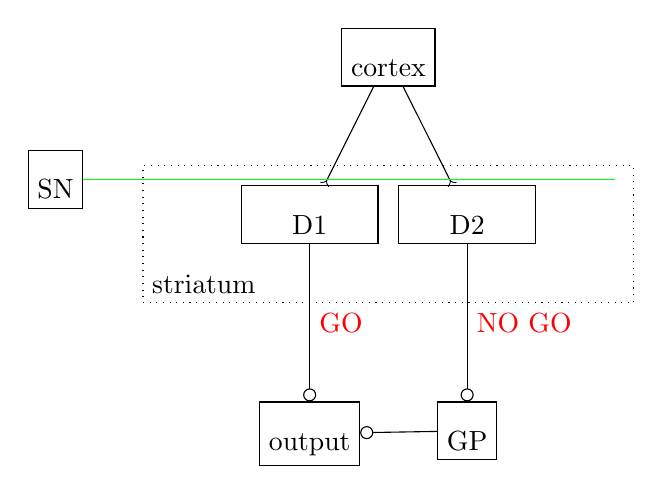
\begin{tikzpicture}
\node[rectangle,draw=black,text height=0.5cm](cortex){cortex};
\node[below = 1.5cm of cortex](v){};
\node[align=left,text height=1.5cm,text width=6cm,rectangle,draw=black,dotted,below = 1cm of cortex](striatum){striatum};
\node[align=center,text height=0.5cm,text width=1.5cm,rectangle,draw=black,left of = v](D1){D1};
\node[align=center,text height=0.5cm,text width=1.5cm,rectangle,draw=black,right of = v](D2){D2};
\draw (cortex) edge[-<] (D1);
\draw (cortex) edge[-<] (D2);
\node[below = 2cm of D1,rectangle,draw=black,text height=0.5cm](output){output};
\draw (D1) edge[-o] node[right,red]{GO} (output);
\node[below = 2cm of D2,rectangle,draw=black,text height=0.5cm](GP){GP};
\draw (D2) edge[-o] node[right,red]{NO GO} (GP);
\draw (GP) edge[-o] (output);
\node [above left = -0.3cm and 2cm of D1,rectangle,draw=black,text height=0.5cm](SN){SN};
\node [above right = -0.3cm and 1cm of D2,text height=0.5cm](SNr){};
\draw (SN) edge[green] (SNr);
\end{tikzpicture}
\end{center}
\caption{Schematic of the go / no-go circuit; the connect from SN through the synapses is a dopamine error signal.\label{fig:gng}}
\end{figure}

In this model the net estimated reward is encoded in the different between the D1 and D2 activity, so
\begin{equation}
m_i=w_i^1 - w_i^2
\end{equation}
where $w_i^1$ and $w_i^2$ are the activity levels, or in this simple
model, equivalently, the synapse strengths, for equivalent D1 and D2
neurons. Although both $w_i^1$ and $w_i^2$ are positive the extra
minus, roughly the extra synapse at GP, allows $m_i$ to be positive or
negative. To learn this, the model suggests the D1 and D2 cells react
differently to dopamine so that
\begin{equation}
w_i^1\rightarrow w_i^1+\eta \delta
\end{equation}
as before, but 
\begin{equation}
w_i^2\rightarrow w_i^2-\eta \delta
\end{equation}
This is not completely outrageous, it is known that dopamine can have
opposite effects on different synapses depending on their receptors,
this is the sort of complicated dynamics that neuromodulators support.

This model predicts that a change in dopamine level will have
different effects on different circuits, it will increase the strength
of the go circuit but decrease the strength of the no-go circuit and
the other way around if the dopamine level is decreased. Hence,
learning from rewards should be facilitated in people with increased
dopamine and learning from punishment from people with decreased
dopamine.

This was tested in \cite{FrankEtAl2004a} using subjects with
Parkinson's disease. People suffering from Parkinson's disease have a
decreased level of dopamine because dopaminergic neurons in SN have
died; one of the main therapies is to give medication which increases
the dopamine level. This makes it possible to manipulate the dopamine
levels of Parkinson's disease by adjust the level of medication;
obviously this relies on the generosity of Parkinson's suffers in
participating in experiments which will involve a temporary increase
in the severity of their symptoms as their medication is
withdrawn. This has been tested using a one-armed-bandit style game,
with happy-face pictures acting as rewards and frowny-face pictures as
punishments; the predicted effect is observed.


\begin{thebibliography}{10}

\bibitem{DawEtAl2006a}
Daw ND, O'Doherty JP, Dayan P, Seymour B and Dolan RJ. (2006) Cortical substrates for exploratory decisions in humans. 
\newblock Nature, 441: 876--879.

\bibitem{ZaghloulEtAl2009a}
Zaghloul KA, Blanco JA, Weidemann CT, McGill K, Jaggi JL, Baltuch GH and Kahana MJ. (2009) Human substantia nigra neurons encode unexpected financial rewards. 
\newblock Science, 323: 1496--1499.

\bibitem{ReynoldsHylandWickens2001a}
Reynolds JN, Hyland BI and Wickens JR. (2001) A cellular mechanism of reward-related learning. 
\newblock Nature, 413: 67--70.

\bibitem{ODohertyEtAl2004a}
O'Doherty J, Dayan P, Schultz J, Deichmann R, Friston K and Dolan RJ. (2004) Dissociable roles of ventral and dorsal striatum in instrumental conditioning. 
\newblock Science, 304: 452--454.

\bibitem{FrankEtAl2004a}
Frank MJ, Seeberger LC and O'Reilly RC. (2004) By carrot or by stick: cognitive reinforcement learning in parkinsonism. 
\newblock Science, 306: 1940--1943.

\end{thebibliography}

\end{document}
